\chapter{Inequalities Revisited}
We finally will now learn about some more advanced methods of solving inequalities ans summations. The last 90 to 100 pages, while essential in their own right, were mostly so that we can do this.\\
\section{Rearrangement Inequalities}
\begin{theorem}
    [Rearrangement Inequality] 
    If $a_1 \geq \dots \geq a_n$ and $b_1 \geq \dots \geq b_n$ then for any permutation (rearrangement) $c_1, \dots, c_n$ of $b_1, \dots, b_n$,\\
$a_1b_n + \dots + a_nb_1 \leq a_1c_1 +\dots +a_nc_n \leq a_1b_1 + \dots + anbn$
\end{theorem}
\begin{proof}
The proof of the Rearrangement Inequality can be handled with proof by contradiction. We will prove the maximization first, the minimization will follow from that.\\
Let us first consider the case where $n=2$. We can take $a_1 \geq a_2$ and $b_1\geq b_2$.\\
$\therefore (a_1-a_2)(b_1-b_2) \geq 0\\
\iff a_1b_1+a_2b_2-a_1b_2-a_2b_1 \geq 0\\
\iff a_1b_1+a_2b_2 \geq a_1b_2+a_2b_1\\$\\
Now for the general case. Let $a_1 \geq a_2 \geq \cdots \geq a_n$ and $b_1 \geq b_2 \geq \cdots \geq b_n$; and let's to the contrary assume that in the grouping maximizing the sum, $a_m$ is not paired with $b_m$. We'll instead assume that $a_m$ is paired with $b_l$ and $b_m$ is paired with $a_l$.\\
Hence we are claiming, $a_mb_l+a_lb_m \geq a_mb_m+a_lb_l$ which is untrue as we showed above.\\
The minimization equality can be very easily proved by noting that if we have the set $\{-b_1, -b_2, \dots -b_n\}$, ordered in increasing order(which makes $b_1 \geq b_2 \geq b_3 \dots \geq b_n)$ and the set $\{a_1, a_2, \ldots\}$, ordered in decreasing order, then the maximum sum is just $-a_1b_n - a_2b_{n-1} + \dots$. Whose negative is $a_1b_n + \dots + a_nb_1$ which will be the minimum possible value.\\ 
\end{proof}
A more refined form of the rearrangement inequality is\\
\begin{theorem}
    [Chebyshev’s Inequality]
     if $a_1\geq a_2\geq ... \geq a_n$ and $b_1\geq b_2\geq ... \geq b_n$ then the following inequality holds:\\
$n \left(\sum_{i=1}^{n}a_ib_i\right)\geq\left(\sum_{i=1}^{n}a_i\right)\left(\sum_{i=1}^{n}b_i\right)$.\\
On the other hand, if $a_1\geq a_2\geq ... \geq a_n$ and $b_n\geq b_{n-1}\geq ... \geq b_1$ then: \\
$n \left(\sum_{i=1}^{n}a_ib_i\right)\leq\left(\sum_{i=1}^{n}a_i\right)\left(\sum_{i=1}^{n}b_i\right)$.
\end{theorem}
\begin{proof}
    The proof is simple. We know that $\sum^n_{i=1}a_ib_i$ is maximal.\\
    $\therefore \sum_{i=1}^{n}a_ib_i\geq a_1b_1+a_2b_2+...+a_n b_{n}$\\
    $\sum_{i=1}^{n}a_ib_i\geq a_1b_2+a_2b_3+...+a_nb_1$\\
    $\vdots$\\
    $\sum_{i=1}^{n}a_ib_i\geq a_1b_n+a_2b_1+...+a_nb_{n-1}$\\
    Adding them will give us the inequality.
\end{proof}
These two inequalities make quick work of even IMO problems. Case in point:\\
\begin{example}
(IMO 1975)
    Let $x_i, y_i~(i = 1, 2, \ldots, n)$ be real numbers such that\[x_1 \geq x_2 \geq \cdots \geq x_n \text{ and } y_1 \geq y_2 \geq \cdots \geq y_n.\]Prove that, if $z_1, z_2, \cdots, z_n$ is any permutation of $y_1, y_2, \cdots, y_n$, then\[\sum_{i=1}^n (x_i - y_i)^2 \leq \sum_{i=1}^n (x_i - z_i)^2.\]
\end{example}
\begin{proof}
    To the untrained eye, this seems quite bad. But let's expand.\\
    $\sum_{i=1}^n (x_i - y_i)^2 \leq \sum_{i=1}^n (x_i - z_i)^2.$\\
    $\iff \sum_{i=1}^n (x_i^2 + y_i^2-2x_iy_i) \leq \sum_{i=1}^n (x_i^2 + z_i^2 - 2x_iz_i)$ as $y_1^2+\dots+y_n^2=z_1^2+\dots+z_n^2$ due to the fact that $z$ is just a rearrangement of $y$.\\
    $\iff \sum_{i=1}^n -2x_iy_i \leq \sum_{i=1}^n - 2x_iz_i\\
    \iff \sum_{i=1}^n x_iy_i \geq \sum_{i=1}^n x_iz_i\\$ which is just the rearrangement inequality. And we are done\\
\end{proof}
\section{Inequalities in Arbitrary Functions}
Till now our inequalities dealt in well understood functions like square, cube, average, reciprocal etc. But what about when the inequality deals in a function like $\sin(x)$ or $\ln{x}$ or maybe $\sin(\ln{x})$, what do we do now?\\
Before we look at the actual inequalities, we'll define two new terms.\\
\begin{definition}
   A convex function is a continuous function whose value at the midpoint of every interval in its domain does not exceed the arithmetic mean of its values at the ends of the interval.
\end{definition}
\begin{definition}
    A concave function is the opposite of a convex function, i.e. a function $f$ is concave if and only if $-f$  is convex.\\
    Basically, A concave function is a continuous function whose value at the midpoint of every interval in its domain exceeds the arithmetic mean of its values at the ends of the interval.
\end{definition}
A simple way to remember is that happy face is convex, while a sad face is concave. \begin{figure}[h]
    \centering
    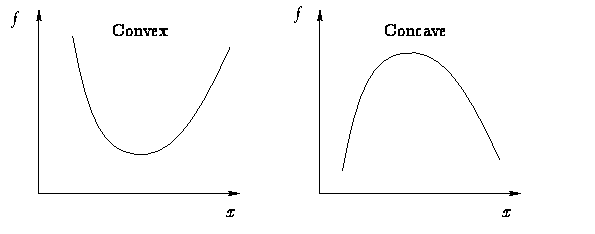
\includegraphics[width=0.75\linewidth]{Photos/convex, concave.png}
    \caption{Convex and Concave graphs}
\end{figure}
We can basically remember that happy face is convex and sad face is concave.\\
For a function, whose graph is harder to plot, we define a function as convex if  $f''(x)\geq 0$ and concave if $f''(0) \leq 0$. This allows us to talk about two more powerful inequalities\\
\begin{theorem}
    [Jensen Inequality]
Let ${F}$ be a convex function of one real variable. Let $x_1,\dots,x_n\in\mathbb R$ and let $a_1,\dots, a_n\ge 0$ satisfy $a_1+\dots+a_n=1$. Then\\
$F(a_1x_1+\dots+a_n x_n)\le a_1F(x_1)+\dots+a_n F(x_n)$\\
If ${F}$ is a concave function, the inequality reverses.
\end{theorem}
\begin{proof}
We only prove the case where $F$ is concave. The proof for the other case follows from the fact that $-F$ is convex.\\ 
Let $\bar{x}=\sum_{i=1}^n a_ix_i$. As $F$ is concave, its slope $F'$ is decreasing. We consider two cases.
If $x_i \le \bar{x}$, then\[\int_{x_i}^{\bar{x}} F'(t) \, dt \ge \int_{x_i}^{\bar{x}} F'(\bar{x}) \, dt .\]
If $x_i > \bar{x}$, then\[\int_{\bar{x}}^{x_i} F'(t) \, dt \le \int_{\bar{x}}^{x_i} F'(\bar{x}) \, dt .\]
By the fundamental theorem of calculus, we have\[\int_{x_i}^{\bar{x}} F'(t) \, dt = F(\bar{x}) - F(x_i) .\]
Evaluating the integrals, each of the last two inequalities implies the same result:\[F(\bar{x})-F(x_i) \ge F'(\bar{x})(\bar{x}-x_i)\]
so this is true for all $x_i$. 
Then we have
\begin{align*} && F(\bar{x})-F(x_i) &\ge F'(\bar{x})(\bar{x}-x_i) \\ \Longrightarrow && a_i F(\bar{x}) - a_i F(x_i) &\ge F'(\bar{x})(a_i\bar{x}-a_i x_i) && \text{as } a_i>0 \\ \Longrightarrow && F(\bar{x}) - \sum_{i=1}^n a_i F(x_i) &\ge F'(\bar{x})\left(\bar{x} - \sum_{i=1}^n a_i x_i \right) && \text{as } \sum_{i=1}^n a_i = 1 \\ \Longrightarrow && F(\bar{x}) &\ge \sum_{i=1}^n a_i F(x_i) && \text{as } \bar{x}=\sum_{i=1}^n a_ix_i \end{align*}as desired.
\end{proof}
We need to note that the weighted AM-GM follows from this.\\
Also we can rewrite Jensen as $\frac{f(a_1)+\dots+f(a_n)}{n} \geq f(\frac{a_1+\dots+a_n}{n})$ for $f$ is convex and reverse if $f$ is convex.\\
\begin{theorem}
    [Karamata's Inequakity]
    If $f$ is convex and $(x_n)$ majorizes $(y_n)$ then:\\
    $f(x_1)+\dots+f(x_n) \geq f(y_1)+\dots+f(y_n)$\\
    The reverse inequality hold true when $f$ is concave.\\
\end{theorem}
\begin{proof}
We will use the fact that $\frac{f(x)-f(y)}{x-y}$ or the slope of graph is decreasing when it is convex. Also using the fact that addition is commutative, we can, without loss of generality assume that $x_1\geq x_2 \geq \dots \geq x_n$ and $y_1\geq y_2 \geq \dots \geq y_n$.\\
We can use that to say: $c_{i+1}=\frac{f(x_{i+1})-f(y_{i+1})}{x_{i+1}-y_{i+1}} \leq \frac{f(x_{i})-f(y_{i})}{x_{i}-y_{i}}=c_i$\\
We will also define $A_i=x_1+\dots+x_i$ and $B_i=y_1+\dots+y_i$
\[\begin{aligned}\sum _{i=1}^{n}{\bigl (}f(x_{i})-f(y_{i}){\bigr )}&=\sum _{i=1}^{n}c_{i}(x_{i}-y_{i})\\&=\sum _{i=1}^{n}c_{i}{\bigl (}\underbrace {A_{i}-A_{i-1}} _{=\,x_{i}}{}-(\underbrace {B_{i}-B_{i-1}} _{=\,y_{i}}){\bigr )}\\&=\sum _{i=1}^{n}c_{i}(A_{i}-B_{i})-\sum _{i=1}^{n}c_{i}(A_{i-1}-B_{i-1})\\&=c_{n}(\underbrace {A_{n}-B_{n}} _{=\,0})+\sum _{i=1}^{n-1}(\underbrace {c_{i}-c_{i+1}} _{\geq \,0})(\underbrace {A_{i}-B_{i}} _{\geq \,0})-c_{1}(\underbrace {A_{0}-B_{0}} _{=\,0})\\&\geq 0,\end{aligned}\]
The proof for concave is similar.\\
\end{proof}
Note that both the proofs are only given for completeness. You can clearly get away with not memorizing them as long as you know the actual inequality.\\
And here is a question from the IMO shortlist to show how powerful inequalities become:\\
\begin{example}
    (IMOSL 2009)  
Given $a + b + c = \frac{1}{a}+\frac{1}{b}+\frac{1}{c}$, Prove that $\frac{1}{(2a+b+c)^2}+\frac{1}{(a+2b+c)^2}+\frac{1}{(a+b+2c)^2} \leq \frac{3}{16}$
\end{example}
\begin{proof}
    Using the fact that $a + b + c = \frac{1}{a}+\frac{1}{b}+\frac{1}{c} \iff \frac{\frac{1}{a}+\frac{1}{b}+\frac{1}{c}}{a + b + c} = 1$\\
    $\frac{1}{(2a+b+c)^2}+\frac{1}{(a+2b+c)^2}+\frac{1}{(a+b+2c)^2} \leq \frac{3}{16} \cdot \frac{\frac{1}{a}+\frac{1}{b}+\frac{1}{c}}{a + b + c}$\\
    As the inequality is homogeneous, we can set $a+b+c=3$\\
    This leaves us with:\\
    $\sum_{cyc} \frac{1}{(3+a)^2} \leq \sum_{cyc} \frac{1}{16a}\\
    \iff 0 \leq \sum_{cyc} \frac{1}{16a}-\frac{1}{(3+a)^2}$\\
    We define $f(x)=\frac{1}{16x}-\frac{1}{(3+x)^2}$, which is convex.\\
    Then using Jensen, $\frac{1}{16a}-\frac{1}{(3+a)^2}+\frac{1}{16b}-\frac{1}{(3+b)^2}+\frac{1}{16c}-\frac{1}{(3+c)^2} \geq 3(\frac{1}{16(\frac{a+b+c}{3})}-\frac{1}{(3+\frac{(a+b+c)}{3})^2})$\\
    As $a+b+c=3$,\\
    $\sum_{cyc} \frac{1}{16a}-\frac{1}{(3+a)^2} \geq 3(\frac{1}{16}-\frac{1}{4^2})$\\
    Which gives us\\
    $\sum_{cyc} \frac{1}{16a}-\frac{1}{(3+a)^2} \geq 0$\\
    Which proves the inequality.\\
\end{proof}
\section{Tangent Line Trick}
For some homogeneous inequality, if we can prove that the function is above the tangent line at the equality value for the sum being $1$, we can prove the inequality by summation.\\
This explanation seems more complicated than the trick actually is. Here is a question to try it out\\
\begin{example}
(USAMO 2003) Let $a$, $b$, $c$ be positive real numbers. Prove that

$\dfrac{(2a + b + c)^2}{2a^2 + (b + c)^2} + \dfrac{(2b + c + a)^2}{2b^2 + (c + a)^2} + \dfrac{(2c + a + b)^2}{2c^2 + (a + b)^2} \le 8.$
\end{example}
\begin{proof}
Since, the inequality is homogeneous we may assume that $a+b+c=1$ and $0<a,b, c<1$.\\
The first time on the LHS is the inequality will be:
\[f(a)=\frac{(a+1)^2}{2a^2+(1-a)^2}=\frac{a^2+2a+1}{3a^2-2a+1}\]
Note that equality holds when $a=b=c=1/3$.\\
We can differentiate to git that the tangent has the equation of the form $y=\frac{12x+4}{3}$.\\
So we claim that
\[f(a) = \frac{a^2+2a+1}{3a^2-2a+1} \leq \frac{12a+4}{3} \text{ for } 0 <a <1\]
Upon clearing the denominators, it is equivalent to:
\[36a^3-15a^2-2a+1 \geq 0\]
Note that since the curve and the line intersect at $1/3, 3a-1$ would be a factor.
\[36a^3-15a^2-2a+1 = (3a-1)^2(4a+1) \geq 0 \text{ for } 0<a<1\]
Adding the similar inequalities for $b$ and $c$ gives:
\[f(a)+f(b)+f(c) \leq \frac{12(a+b+c) +12}{3} = 8\]
\end{proof}
While I recommend trying Jensen and Karamarta before pulling out the Tangent Trick. However, when nothing else works, kill with calc.\\
\section{SEBACS Generalized}
\begin{theorem}
    [Holder's Inequality]
    If $a_1, a_2, \dotsc, a_n, b_1, b_2, \dotsc, b_n, \dotsc, z_1, z_2, \dotsc, z_n$ are non-negative real numbers and $\lambda_a, \lambda_b, \dotsc, \lambda_z$ are non-negative reals with sum of 1, then\[(a_1 + \dotsb + a_n)^{\lambda_a} (b_1 + \dotsb + b_n)^{\lambda_b} \dotsm (z_1 + \dotsb + z_n)^{\lambda_z} \geq a_1^{\lambda_a}b_1^{\lambda_b} \dotsm z_1^{\lambda_z} + \dotsb + a_n^{\lambda_a}b_n^{\lambda_b} \dotsm z_n^{\lambda_z}.\]
Note that with two sequences $\mathbf{a}$ and $\mathbf{b}$, and $\lambda_a = \lambda_b = 1/2$, this is SEBACS inequality.
\end{theorem}
\begin{proof}
    This is one the most easy proof in this book. We need to notice that $(a_1 + \dotsb + a_n), (b_1 + \dotsb + b_n), \dotsm, (z_1 + \dotsb + z_n)$ are homogeneous, allowing us to take $a_1+\dots+a_n=b_1+\dots+b_n=\dots=z_1+\dots+z_n=1$, converting the inequality to:\\
    $1 \geq a_1^{\lambda_a}b_1^{\lambda_b} \dotsm z_1^{\lambda_z} + \dotsb + a_n^{\lambda_a}b_n^{\lambda_b} \dotsm z_n^{\lambda_z}$\\
    Which is trivially true as $a_1, a_2, \dotsc, a_n, b_1, b_2, \dotsc, b_n, \dotsc, z_1, z_2, \dotsc, z_n$ are non-negative real numbers.
\end{proof}
However, sadly SEBACS tends to be used more often. Also I am yet to see any inequality which can be done by Holder but not using Jensen or Karmata. However, here is an example(which can be done using Jensen, and I encourage you to do that)\\
\begin{example}
    Let $a,b,c$ be positive real numbers. Prove that $\frac{a}{\sqrt{a^{2}+8bc}}+\frac{b}{\sqrt{b^{2}+8ca}}+\frac{c}{\sqrt{c^{2}+8ab}}\ge 1$.
\end{example}
\begin{proof}
    Jensen does this using $abc=1$ and then the question dies in silence\\
    However, for Holder, we'll need to 'observe' that:\\
    $a(a^2+8bc) \cdot (\frac{a}{\sqrt{a^2+8bc}})^2= a^3$\\
    Which we can use to say, using Holder:\\
    $\sum_{cyc} a(a^2+8bc) \cdot \sum_{cyc}(\frac{a}{\sqrt{a^2+8bc}})^2 \geq \sum_{cyc} a^3\\
    \iff \sum_{cyc} (a(a^2+8bc))^{\frac{1}{3}} \cdot \sum_{cyc}((\frac{a}{\sqrt{a^2+8bc}}))^{\frac{2}{3}} \geq a+b+c$\\
    Which will change our to prove to:\\
    $(a+b+c)^3 \geq \sum_{cyc} a(a^2+8bc)\\
    \iff a^3+b^3+c^3+3(a+b)(b+c)(c+a) \geq a^3+b^3+c^2+24abc\\
    \iff 3(a+b)(b+c)(c+a) \geq 24abc\\
    \iff (a+b)(b+c)(c+a) \geq 8abc$\\
    Notice that $a+b \geq 2\sqrt{ab}$ and similar for the others, leading to the multiplication:\\
    $(a+b)(b+c)(a+c) \geq 2\sqrt{ab} \cdot2\sqrt{bc} \cdot2\sqrt{ac}\\
    \iff (a+b)(b+c)(a+c) \geq 8\sqrt{a^2b^2c^2}\\
    \iff (a+b)(b+c)(a+c) \geq 8abc$\\
\end{proof}
\section{Lagrange Multipliers}
This is the most powerful trick/method/theorem about inequalities. This is the reason why I can solve almost any inequality in an instant. Is this almost cheating? YES. Is it allowed if you write it up correctly? YES!\\
Lagrange multiplier finds the extreme of multi variable functions given a constraint.\\
\begin{example}
    [Motivating Example]
    Maximize $f(x,y)=2x+y$ for $x^2+y^2=1$. 
\end{example}
\begin{proof}
    [Solution]
    Before we go further, I know that this example is doable with basic calculus as well. However, let's try to explore a new technique.\\
    We'll use a concept called gradients($\nabla x$), vectors(lines) which are perpendicular to the tangent of a graph.\\
    This is useful as the extremal value will occur at the point where $f(x,y)=2x+y$ is perpendicular to $g(x,y)=x^2+y^2=1$\\
    \begin{figure} [h]
        \centering
        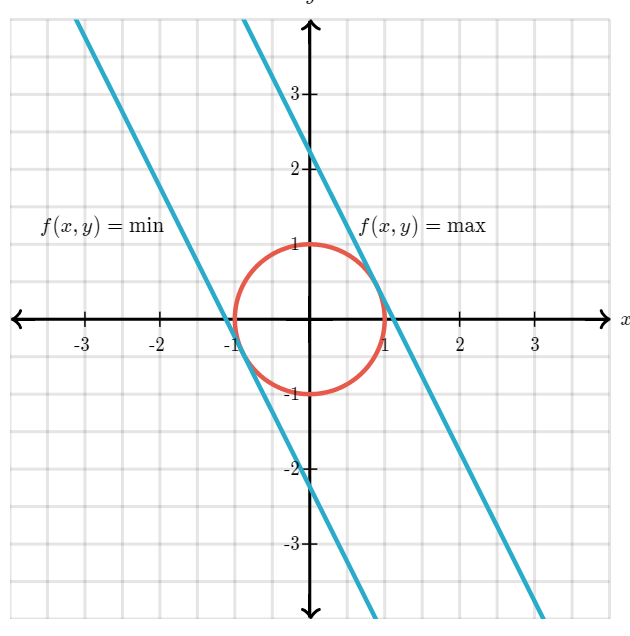
\includegraphics[width=0.5\linewidth]{Photos/Gradient Lagrange.png}
        \caption{The point of maxima and minima}
    \end{figure}
    While in this case the lines are straight, sometimes we end up with a much more curvy line, however the observation holds.\\
    Another key observation to make is that if two graphs are tangent, the gradient lines at point of tangency are parallel. We can therefore say that, $\nabla f(x,y)= \lambda \nabla g(x,y)$ as they are parallel.\\
    We now need to calculate the gradient. The gradient can be written as a column matrix $\begin{bmatrix}
        \frac{\partial f(x,y)}{\partial x}\\
        \frac{\partial f(x,y)}{\partial y}
    \end{bmatrix}$ where $\frac{\partial}{\partial x}$ means the derivative of $f(x,y)$ considering everything else other than $x$ as a constant.\\
    Why does this definition work? That should keep you curios till the Calc III course in collage.\\
    But with this in hand, we can solve our question:\\
    $\begin{bmatrix}
        2\\
        1\\
    \end{bmatrix} = \lambda \begin{bmatrix}
        2x\\
        2y
    \end{bmatrix}$\\
    Using the definition of equal matrices, $2 \lambda x=2; 2\lambda y=1$\\
    Which gives us $x=2y$ which means $4y^2+y^2=1\\
    \iff y=\pm \frac{1}{\sqrt{5}}$\\
    Which means the maxima of $2x+y=5y$ is $\sqrt{5}$ and minima is $-\sqrt{5}$\\
\end{proof}
This may seem excessive, and frankly overkill for the given question, but it becomes increasingly more powerful as we look at Olympiad questions. We basically partial differentiate both the functions and declare their ratio as $\lambda$. This along with the original equation leads to the maxima or minima, which solves the inequality.\\
Be very careful while using it as it will attract the wrath of the grader as it is an undergraduate method. However, if we are careful, it is also free marks. This is at the end to discourage you from only using Lagrange(like I did for quite a long time) and use the actual inequalities.\\
Everytime we have an inequality question, we can do it by the others as well. Just that Lagrange is easier and quicker most of the times. Here is an example from MOP, to put a close on inequalities\\
\begin{example}
(MOP 2012)
Given that $a + b + c + d = 4$, for positive reals $a, b, c, d$ prove that\\
$\frac{1}{a^2}+\frac{1}{b^2}+\frac{1}{c^2}+\frac{1}{d^2} \geq a^2+b^2+c^2+d^2$
\end{example}
\begin{proof}
    While this can be done using Tangent line, Jensen and more, we'll use Lagrange.\\
    We'll rewrite the inequality as: $\frac{1}{a^2}-a^2+\frac{1}{b^2}-b^2+\frac{1}{c^2}-c^2+\frac{1}{d^2}-d^2 \geq 0$
    $\begin{bmatrix}
        1\\
        1\\
        1\\
        1\\
    \end{bmatrix} = \lambda \begin{bmatrix}
        \frac{-2}{a^3}-2a\\
        \frac{-2}{b^3}-2b\\
        \frac{-2}{c^3}-2d\\
        \frac{-2}{d^3}-2d\\
    \end{bmatrix}$\\
    We can notice that $a=b=c=d=\frac{4}{4}=$1 at the minima which is $0$. This makes the inequality true\\
    NOTE: If you are rigorous, you may notice that we don't know if $0$ is the maxima or the minima. In this case we can test it by having two variables(and rest as $1$s) and proving that it is always above $0$. This while still not the correct way, is satisfactory(as this is almost similar to the single derivative test). The more accurate methods of determining this will come in undergraduate studies. 
\end{proof}
\section{Sum uses of Calc}
\begin{example}
    [Motivating Example]
    For a polynomial $p(x)$ with roots $r_1,r_2,r_3 \dots r_n$ find:\\
    \[\sum^n_{i=1}\frac{1}{x-r_i}\]
\end{example}
\begin{proof}
    [Solution]
    While we can do this using vieta, here is the most chad way of going about it.\\
    We know that $p(x)=a(x-r_1)(x-r_2)\dots(x-r_n)$\\
    We can convert it to sum by taking log $\log{p(x)}=\log{a}+\log{x-r_1}+\dots+\log{x-r_n}$\\
    We can convert it into reciprocals by diffrentiation:\\
    $\frac{p'(x)}{p(x)}=\frac{1}{x-r_1}+\frac{1}{x-r_2}+\dots +\frac{1}{x-r_n}$\\
    This solves the question.
\end{proof}
As we can see, discrete summations can also be done using analytic techniques(calc). However, the fun part is almost all discrete sums are solvable by these methods.\\
However, we'll make a few assumptions about the question before solving them. While this may seem wrong, here is an assumption we have been making for quite some time:\\
$1-1+1-1+\dots$\\
Some of you may compute this as $(1-1)+(1-1)+\dots =0$ or you may compute this as $1+(-1+1)+(-1+1)\dots =1$ or in the correct way as an infinite GP $\frac{1}{1-(-1)}=\frac{1}{2}$.\\
The other two are wrong as the given series is conditionally convergent(converges in only a few cases, and diverges in other, definition wise has the absolute sum of terms diverging) which makes grouping inherently wrong. The Riemann Series theorem(which you'll learn more about in real analysis, not in this book) proves that this is not allowed. However, we have been rearranging and grouping sums for quite a long time without running into any such issues.\\
This is because we are assuming that that the series is absolutely convergent(converges all the time). This allows grouping, order changes and all the other techniques.\\
We'll now with the knowledge about our ignorance, proceed to ignore it once more as questions are questions as the series is absolutely convergent.\\
You will study more about conditional convergence in real analysis and discrete analysis courses.\\
\begin{definition}
A power series (centered at 0) is an infinite series of the form\\
\[\sum^{\infty}_{n=0} a_nz^n=a_0+a_1z+a_2z^2+\dots \]
where $a_i \in \mathbb{C}$ for all $i \geq 0$.
\end{definition}
While it is hard to see whether every such series converges, however here is a simple way to check:\\
\begin{definition}
    \[R = (\limsup_{n \to \infty}|a_n|^{\frac{1}{n}})^{-1}\]
    Here $\limsup$ refers to the maximum possible value of the function at the limit. Basically, for a function like $\sin$ this refers to $1$ at $\infty$ as otherwise it's an oscillating limit.\\
    \begin{figure} [h]
        \centering
        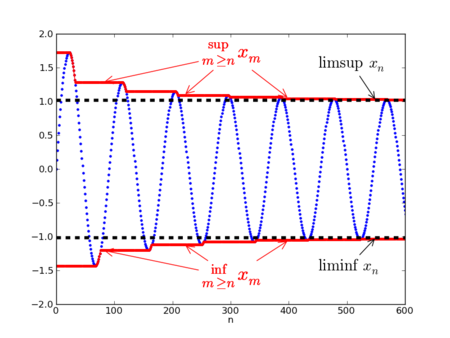
\includegraphics[width=0.5\linewidth]{Photos/Limsup.png}
        \caption{$\limsup$ and $\liminf$ in a graph}
    \end{figure}
    Here $R$ is the radius of convergence. The series converges(normally) if $z: |z| < R$ and diverges to $\infty$ or $-\infty$ if $z: |z| > R$.
\end{definition}
We'll not use this again. It's useless in most cases. As I said before, we normally assume a series is absolutely convergent.\\
We should also remember the Taylor series expansions, as we are going to use them.\\
\begin{example}
    \[\sum^{\infty}_{n=0} \frac{1}{(2n)!!}\]
    where $n!! = n(n-2)(n-4) \dots$ is the double factorial.\\
\end{example}
\begin{proof}
    [Solution]
$\sum^{\infty}_{n=0} \frac{1}{(2n)!!}\\
\sum^{\infty}_{n=0} \frac{1}{(2n)(2n-2)(2n-4)\dots(2)}\\
\sum^{\infty}_{n=0} \frac{1}{2^n(n)(n-1)(n-2)\dots(1)}\\
\sum^{\infty}_{n=0} \frac{1}{2^n n!}\\
\sum^{\infty}_{n=0} \frac{\frac{1}{2^n}}{n!}\\
$
Which is the Taylor series for $e^{\frac{1}{2}}=\sqrt{e}$.\\
\end{proof}
Here is also another fun fact:\\
\begin{theorem}
    [Differentiating and integrating under the power series]
    For 'well behaved' function, we can say if:\\
    \[F(x)=\sum^{\infty}_{n=0}a_nx^n\]
    then:\\
    \[F'(x)=\sum^{\infty}_{n=1}(n-1)a_nx^{n-1}\]
    and:\\
    \[\int F(x) dx = \sum^{\infty}_{n=0}a_n \frac{x^{n+1}}{n+1}\]
    Basically, as long as our functions are well behaved, we differentiate and integrate them term by term.\\
    This can also be used to say, for a well behaved function:\\
    \[int \sum f(x)= \sum \int f(x)\]
\end{theorem}
We will use these properties to solve the follwong example:\\
\begin{example}
(AMSP) Prove that    \[ \sum^n_{r=1} \frac{1}{r} \binom{n}{r}= \sum^n_{r=1} \frac{2^r-1}{r}\]
for $n \in \mathbb{Z^+}$
\end{example}
\begin{proof}
    We will use the rewrite $\frac{1}{r} =\int^1_0 x^{r-1} dx$, using this on the LHS gives us:\\
    $
    \sum^n_{r=1} \binom{n}{r} \int^1_0 x^{r-1} dx\\
    \int^1_0 \sum^n_{r=1}  \binom{n}{r} x^{r-1} dx$\\
    This looks an awful lot like the binomial theorem with some modifications.\\
    $\int^1_0 \frac{(1+x)^n-1}{x} dx$\\
    This can be solved by integration by substitution taking $u=x+1$\\
    $\int^2_1 \frac{u^n-1}{u-1} du$\\
    Which using the sum of GP turns to:\\
    $\int^2_1 \sum^n_{r=1}u^{r-1} dr\\
    \sum^n_{r=1} \int^2_1 u^{r-1} dr\\
    \sum^n_{r=1} \frac{2^r-1}{r}$\\
    Which proves the above.\\
\end{proof}
\begin{xcb} {Exercises}
    \begin{enumerate}
\item  Let $a,b,c,d$ be positive real numbers with $a+b+c+d=1$. Prove that:\\
$6(a^3+b^3+c^3+d^3) \geq a^2+b^2+c^2+d^2+\frac{1}{8}$
\item (USAMO 1978) Given that $a, b, c, d, e$ are real numbers such that $a + b + c + d + e = 8$\\
$a^2 + b^2 + c^2 + d^2 + e^2 = 16$
determine the minimum value of $e$.
\item (Canada 1997)  Prove that for non negative real numbers $a, b, c$ with $a + b + c = 1$ we have\\
$a^2b + b^2c + c^2a \leq \frac{4}{27}$
\item (USAMO 2011) If $a^2 + b^2 + c^2 + (a + b + c)^2 \leq 4$, then\\
\[\frac{1+ab}{(a+b)^2}+\frac{1+bc}{(b+c)^2}+\frac{1+ac}{(a+c)^2} \geq 3\]\\
\item Let $a, b, c$ be positive reals satisfying $a + b + c = \sqrt[7]{a}+\sqrt[7]{b}+\sqrt[7]{c}$.  Prove that $a^a b^bc^c \geq 1$
\item Let $a,b,c$ be the sides of a triangle. Prove that:\\
$\frac{a}{b+c-a}+\frac{a}{b+c-a}+\frac{a}{b+c-a} \geq 3$\\
\item Let $a,b,c$ be real numbers such that $0 \leq a,b,c \leq 1$, then prove\\
$\frac{a}{1+bc}+\frac{a}{1+bc}+\frac{c}{1+ab} \leq 2$
\item (USAMO 2004) Let $a$, $b$, and $c$ be positive real numbers. Prove that
$(a^5 - a^2 + 3)(b^5 - b^2 + 3)(c^5 - c^2 + 3) \ge (a+b+c)^3$.
\end{enumerate}
\end{xcb}